% !TEX TS-program = pdflatex
% !TEX encoding = UTF-8 Unicode

% This is a simple template for a LaTeX document using the "article" class.
% See "book", "report", "letter" for other types of document.

\documentclass[11pt]{article} % use larger type; default would be 10pt

\usepackage[utf8]{inputenc} % set input encoding (not needed with XeLaTeX)

%%% Examples of Article customizations
% These packages are optional, depending whether you want the features they provide.
% See the LaTeX Companion or other references for full information.

%%% PAGE DIMENSIONS
\usepackage{geometry} % to change the page dimensions
\geometry{a4paper} % or letterpaper (US) or a5paper or....
% \geometry{margin=2in} % for example, change the margins to 2 inches all round
% \geometry{landscape} % set up the page for landscape
%   read geometry.pdf for detailed page layout information

\usepackage{graphicx} % support the \includegraphics command and options
\usepackage[parfill]{parskip} % Activate to begin paragraphs with an empty line rather than an indent

%%% PACKAGES
\usepackage{booktabs} % for much better looking tables
\usepackage{array} % for better arrays (eg matrices) in maths
\usepackage{paralist} % very flexible & customisable lists (eg. enumerate/itemize, etc.)
\usepackage{verbatim} % adds environment for commenting out blocks of text & for better verbatim
\usepackage{subfig} % make it possible to include more than one captioned figure/table in a single float
% These packages are all incorporated in the memoir class to one degree or another...

%%% HEADERS & FOOTERS
\usepackage{fancyhdr} % This should be set AFTER setting up the page geometry
\pagestyle{fancy} % options: empty , plain , fancy
\renewcommand{\headrulewidth}{0pt} % customise the layout...
\lhead{}\chead{}\rhead{}
\lfoot{}\cfoot{\thepage}\rfoot{}

%%% SECTION TITLE APPEARANCE
\usepackage{sectsty}
\allsectionsfont{\sffamily\mdseries\upshape} % (See the fntguide.pdf for font help)
% (This matches ConTeXt defaults)

%%% ToC (table of contents) APPEARANCE
\usepackage[nottoc,notlof,notlot]{tocbibind} % Put the bibliography in the ToC
\usepackage[titles,subfigure]{tocloft} % Alter the style of the Table of Contents
\renewcommand{\cftsecfont}{\rmfamily\mdseries\upshape}
\renewcommand{\cftsecpagefont}{\rmfamily\mdseries\upshape} % No bold!


\usepackage{algorithmicx}
\usepackage{algpseudocode}


%%% END Article customizations

%%% The "real" document content comes below...

\title{Project Progress Report}
\author{Jiachi Liu \& Peili Cao}
%\date{} % Activate to display a given date or no date (if empty),
         % otherwise the current date is printed 

\begin{document}
\maketitle

\section{Data Description}
\subsection{K-means}

For K-Means major task, we are using MillionSongs dataset to divide songs into K different clusters. Since million songs dataset contains a lot of meta data of music, such as mode, key, segments, we are using a subset of those features to reduce the size of data, which contains 15 features. The features are: artist familiarity, artist hotness, number of similar artists, number of artist terms, duration, end of fade in, key, key confidence, loudness, mode, mode confidence, start of fade out, temp, year, song hotness. Figure \ref{fig:msd} shows some lines of data as example.

\subsection{Frequent itemset mining}

For Frequent itemset mining, we are using Taste Profile subset from MillionSongs dataset. This dataset contains two columns: the first column represents user and the second column represents song. Table \ref{table: stats-taste-dataset} shows the statistics of this dataset.

\begin{figure}[htbp]
\begin{center}
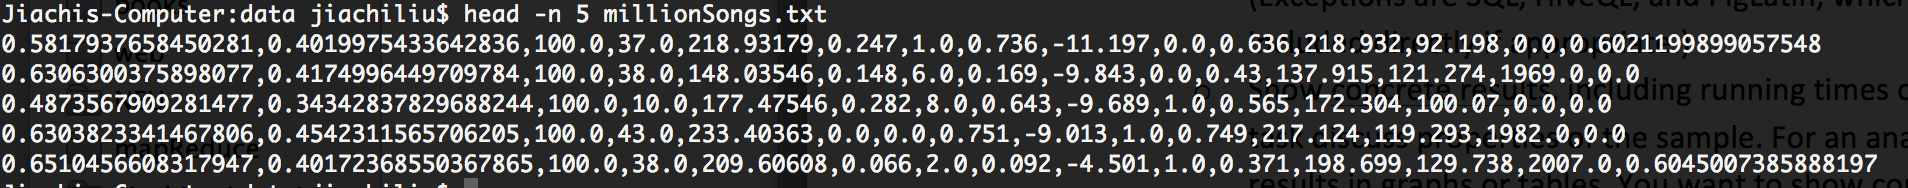
\includegraphics[scale=0.4]{millionsongs.png}
\caption{Million Songs data example}
\label{fig:msd}
\end{center}
\end{figure}

\begin{table}[htdp]
\caption{Statistics of Taste Profile Subset}
\begin{center}
\begin{tabular}{|c|c|c|}
\hline
Unique Users &Unique MSD songs &User-Song-Playcounts Triplets \\ \hline
1,019,318  & 384,546 & 48,373,586\\ \hline
\end{tabular}
\end{center}
\label{table: stats-taste-dataset}
\end{table}%

\section{Task Progress}
\subsection{K-Means}
For K-Means task, we have implemented the distributed version of KMeans and run it on amazon AWS among 10,000 songs.
\subsubsection{Pseudo Code}
The Mapper of KMeans Algorithm will read the current K centroids from HDFS file and save them into the memory in setup function. In map function call, for each line of data, we assign it to the centroid that has minimum distance. The distance is calculated as Euclidean distance between the data point and centroids. The mapper then emits the centroid id as a key and the data point as value.

\begin{algorithmic}[1]
\Function{map}{key, data}
\State $minDistance \gets Infinity$
\State $centroidId = -1$
\For{each centroid $c$ in centroids}
	\State $dist \gets distance(c, data)$
	\If{dist < minDistance}
		\State $minDistance \gets dist$
		\State $centroidId = c.id$
	\EndIf
\EndFor
\State $emit(centroidId, data)$
\EndFunction
\end{algorithmic}

The reducer will update the centroid vector by calculating the average vector among the input data point list. And emit the new centroid to output file.
\begin{algorithmic}[1]
\Function{reduce}{cid, [$d_1,d_2....,d_n$]}
\State $sumVector \gets 0$
\State $count \gets 0$
\For{each data $d$ in input list}
	\State $sumVector +=  d$
	\State $count ++$
\EndFor
\State $newCentroid = sumVector / count$
\State $emit(newCentroid, Null)$
\EndFunction
\end{algorithmic}

The Driver class will repeatedly create map reduce job for each iteration of KMeans. It will first initialize centroids based on input K before start KMeans algorithm, and then start create jobs for each iteration to get new computed centroids. After that, it will copy the output file to currentCentroid folder so the mapper can read current centroids from it. Also, it will delete the output file in order to avoid exceptions on map reduce job. And to stop the iterations, it will read and compute the sum of distance of all centroids between two iterations and determines whether to stop.

\begin{algorithmic}[1]
\Function{isConverge}{oldCentroids, newCentroids}
\State $dist \gets 0$
\For{each old centroids o, and new centroids n}
	\State $dist += distance(o, n)$
\EndFor \\
\Return $dist <= threshold$
\EndFunction
\end{algorithmic}

\subsubsection{Running Result}
Table \ref{table: kmean-running-time-table} shows the running time on AWS for different K.

\begin{table}[htdp]
\caption{K-Means Runtime Table}
\begin{center}
\begin{tabular}{|c|c|c|c|}
\hline
K & \# of Iterations & 5 workers \\ \hline
2 & 2 &	4m01s & 3m32s \\ \hline
3 & 11 &	21m43s & 20m41s\\ \hline
5 &	18 & 38m32s & 34m38s\\ \hline
10 & 32 & 1h09m12s & 1h00m33s	\\ \hline
20 & 58 & 2h30m41s & 2h00m07s	\\ \hline
30 & 76 & 3h52m58s & 2h56m49s	\\ \hline
\end{tabular}
\end{center}
\label{table: kmean-running-time-table}
\end{table}%

\subsection{Frequent itemset mining}
\subsubsection{Preprocessing data}

Since the user-id and song-id provided in original data file are long string, we first replace the data with new sequential id. For user, id starts from 0 to 1,019,317. For song, id starts from 0 to 384,546. After reformatting ids, we need to generate transactions to perform Apriori Algorithm. Figure \ref{fig:new-format-user-song-pair} shows an example of the transactions. Row i represents the list of songs that listened by $user_{i}$. The lists are ordered.

\begin{figure}[htbp]
\begin{center}
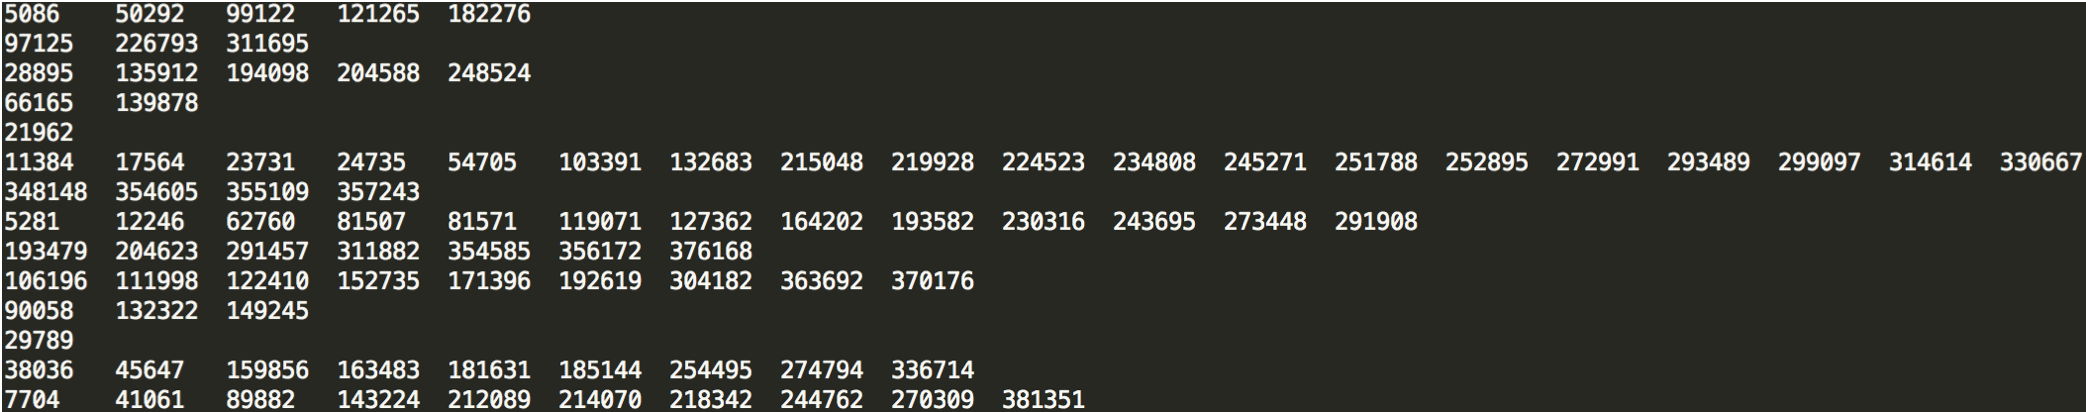
\includegraphics[scale=0.25]{transactions.png}
\caption{Transaction Example}
\label{fig:new-format-user-song-pair}
\end{center}
\end{figure}

\subsubsection{Pseudo Code}
\begin{algorithmic}[1]
\State $itemset_1 \gets  (Size1\_Frequent\_Items)$
\For{$k=1,Itemset_k not empty;k++$}
	\State $candidates_{k+1} = itemset_k\ sort\_join\ itemset_1$
	\For {each transaction t in transactions}
		\State each map will have a copy of $candidates_{k+1}$
		\State $emit(candidates_{k+1},count)$
	\EndFor
	\State //In Reducer 
	\For{each candidate in $candidates_{k+1}$}
		\If{$count >= min\_support$}
			$emit(candidates)$
		\EndIf
	\EndFor
	\State $itemset_{k+1} = reduce\_outputs$
\EndFor

\end{algorithmic}

\subsubsection{Generate Size K Frequent Item Candidate}
To generate size K($K>=2$) frequent item candidates, we join size $K-1$ frequent items with size 1 frequent items. In order to improve efficiency of algorithm, we make sure that ids of size $K-1$ frequent items are in order. There will be two mappers. One is for reading size 1 frequent items, the other is for reading size $K-1$ frequent items. The key of two mappers are $("dummy",tag)$. And Partitioner and GroupComparator will only consider $"dummy"$. 
Pseudo Code \\
\begin{algorithmic}[1]
\Function{map}{offset,value}
\State $emit("dummy",tag,value)$
\EndFunction
\end{algorithmic}
In Reducer, it will store records into two separate lists based on tag and then join the two lists. Since the two lists are all ordered, there will be no duplicates candidates.
\begin{algorithmic}[1]
\Function{reduce}{$"dummy",tag, list of itemsets$}
\For{each item in list}
	\State $TagAList.add(item from A)$
	\State $TagBList.add(item from B)$
\EndFor
\For{each item in A}
	\For{each item in B}
		\State $candidate = join(A.item, B.item)$
		\State $emit(candidate)$
	\EndFor
\EndFor	
\EndFunction
\end{algorithmic}

\subsubsection{Analysis}
We analysis the number of listening users  for each song ids. Table \ref{table: stats-song} shows mean, max, min for all songs. Figure \ref{fig:distr-song} shows the distribution of the number of listening users for each song. We split songid into 20 bins. X coordinates means the number of bin. Y coordinates means the number of songs located in that bin. The scope of first bin is (1,5525)

\begin{table}[htdp]
\caption{Statistics of Taste Profile Subset}
\begin{center}
\begin{tabular}{|c|c|c|}
\hline
Mean & Max & Min \\ \hline
125.79 & 110479 & 1 \\ \hline
\end{tabular}
\end{center}
\label{table: stats-song}
\end{table}%

\begin{figure}[htbp]
\begin{center}
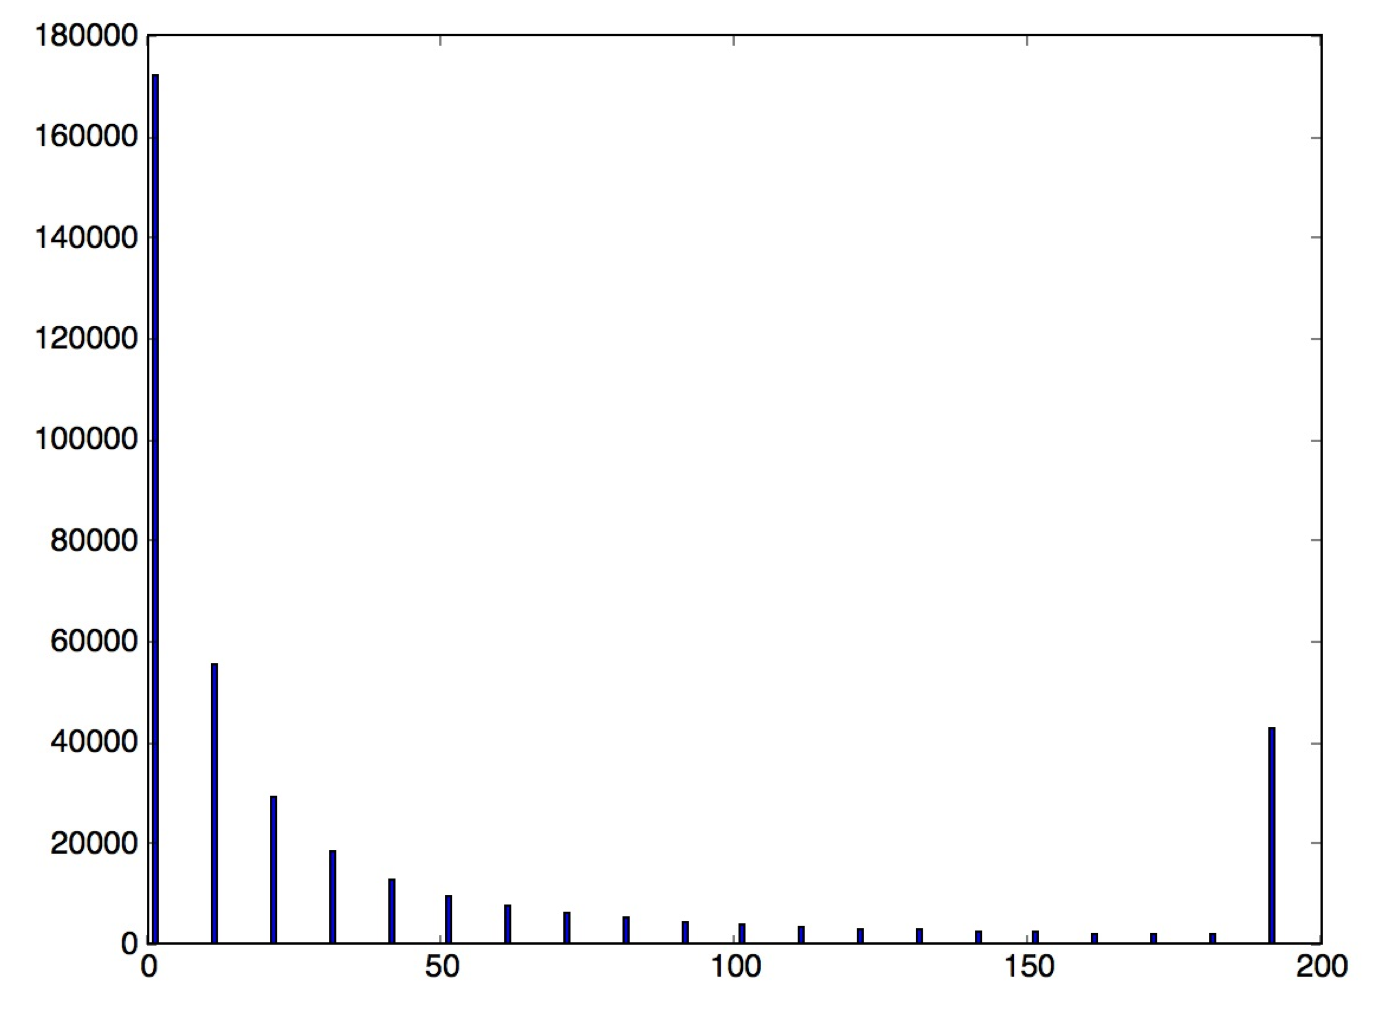
\includegraphics[scale=0.3]{dist_songs.png}
\caption{Distribution of \# of listening users for songs }
\label{fig:distr-song}
\end{center}
\end{figure}


\section{Remain Work}
\begin{itemize}
\item For K-Means problem, we will need a helper task to calculate the Mean Root Square Error between the centroid and songs in same cluster to measuring the quality of the algorithm. And we will also implement a local version K-Means algorithm to compare the performance with distributed version.
\item For Frequent Itemsets, we will continue to implement Apriori Algorithm. Till now, we've implemented generating size1-3 frequent itemset. After implementing, we will run it on AWS. We also notice that there are transactions that can be eliminate when there is no frequent itemset in it, but doing this may make code more complicate. 
\end{itemize}

\end{document}

